% Options for packages loaded elsewhere
\PassOptionsToPackage{unicode}{hyperref}
\PassOptionsToPackage{hyphens}{url}
%
\documentclass[
]{article}
\usepackage{amsmath,amssymb}
\usepackage{iftex}
\ifPDFTeX
  \usepackage[T1]{fontenc}
  \usepackage[utf8]{inputenc}
  \usepackage{textcomp} % provide euro and other symbols
\else % if luatex or xetex
  \usepackage{unicode-math} % this also loads fontspec
  \defaultfontfeatures{Scale=MatchLowercase}
  \defaultfontfeatures[\rmfamily]{Ligatures=TeX,Scale=1}
\fi
\usepackage{lmodern}
\ifPDFTeX\else
  % xetex/luatex font selection
\fi
% Use upquote if available, for straight quotes in verbatim environments
\IfFileExists{upquote.sty}{\usepackage{upquote}}{}
\IfFileExists{microtype.sty}{% use microtype if available
  \usepackage[]{microtype}
  \UseMicrotypeSet[protrusion]{basicmath} % disable protrusion for tt fonts
}{}
\makeatletter
\@ifundefined{KOMAClassName}{% if non-KOMA class
  \IfFileExists{parskip.sty}{%
    \usepackage{parskip}
  }{% else
    \setlength{\parindent}{0pt}
    \setlength{\parskip}{6pt plus 2pt minus 1pt}}
}{% if KOMA class
  \KOMAoptions{parskip=half}}
\makeatother
\usepackage{xcolor}
\usepackage[margin=1in]{geometry}
\usepackage{longtable,booktabs,array}
\usepackage{calc} % for calculating minipage widths
% Correct order of tables after \paragraph or \subparagraph
\usepackage{etoolbox}
\makeatletter
\patchcmd\longtable{\par}{\if@noskipsec\mbox{}\fi\par}{}{}
\makeatother
% Allow footnotes in longtable head/foot
\IfFileExists{footnotehyper.sty}{\usepackage{footnotehyper}}{\usepackage{footnote}}
\makesavenoteenv{longtable}
\usepackage{graphicx}
\makeatletter
\def\maxwidth{\ifdim\Gin@nat@width>\linewidth\linewidth\else\Gin@nat@width\fi}
\def\maxheight{\ifdim\Gin@nat@height>\textheight\textheight\else\Gin@nat@height\fi}
\makeatother
% Scale images if necessary, so that they will not overflow the page
% margins by default, and it is still possible to overwrite the defaults
% using explicit options in \includegraphics[width, height, ...]{}
\setkeys{Gin}{width=\maxwidth,height=\maxheight,keepaspectratio}
% Set default figure placement to htbp
\makeatletter
\def\fps@figure{htbp}
\makeatother
\setlength{\emergencystretch}{3em} % prevent overfull lines
\providecommand{\tightlist}{%
  \setlength{\itemsep}{0pt}\setlength{\parskip}{0pt}}
\setcounter{secnumdepth}{-\maxdimen} % remove section numbering
\ifLuaTeX
  \usepackage{selnolig}  % disable illegal ligatures
\fi
\usepackage{bookmark}
\IfFileExists{xurl.sty}{\usepackage{xurl}}{} % add URL line breaks if available
\urlstyle{same}
\hypersetup{
  pdftitle={iButton Temperature Data from 2021-2023 NIRPO Plots in Prudhoe Bay, Alaska},
  pdfauthor={Jana Peirce},
  hidelinks,
  pdfcreator={LaTeX via pandoc}}

\title{iButton Temperature Data from 2021-2023 NIRPO Plots in Prudhoe
Bay, Alaska}
\author{Jana Peirce}
\date{6 November 2023}

\begin{document}
\maketitle

\subsection{File prep}\label{file-prep}

\begin{itemize}
\tightlist
\item
  Save all data with datetime info in csv before bringing into r (do not
  use readxl package)
\item
  Format all times as yyyy-mm-dd before importing into r
\end{itemize}

\begin{verbatim}
##         Date  Time   T02    T04   T06    T08    T09    T11   T12    T13    T14
## 1 2021-07-31  0:00 4.071 12.072 5.531 11.451 10.642 10.110 5.592 11.610 11.060
## 2 2021-07-31  4:00 4.071 10.571 5.531  9.449  8.634  8.604 5.090 10.105  9.056
## 3 2021-07-31  8:00 4.071 12.072 5.028 11.951 11.645 10.611 5.090 11.108 11.060
## 4 2021-07-31 12:00 3.569 17.077 5.028 20.455 18.664 16.126 5.090 14.117 15.066
## 5 2021-07-31 16:00 3.569 17.077 5.028 18.454 18.664 15.124 5.090 15.119 16.067
## 6 2021-07-31 20:00 4.071 17.077 5.028 18.454 18.163 15.124 5.592 16.122 17.068
##      T17   T19    T20    T21   T22    T23   T24   T25   T26   T27   T28   T29
## 1 10.601 3.564 10.642 12.064 9.075 10.059 6.063 4.047 3.583 6.120 4.573 3.583
## 2  8.096 3.564  8.634 10.560 8.574  8.554 6.063 4.047 3.583 6.120 5.075 3.583
## 3 11.101 3.062 11.144 11.563 7.570 10.560 5.561 4.047 3.583 5.619 5.075 3.583
## 4 17.108 3.062 15.657 14.570 8.072 17.575 5.561 4.047 3.583 5.619 5.075 3.583
## 5 17.108 3.062 16.660 16.072 9.075 17.074 5.561 4.047 3.583 5.619 4.573 3.583
## 6 18.109 3.062 16.660 16.573 9.577 17.074 5.561 4.047 3.583 5.619 4.573 3.583
##      T30   T31    T33   T35   T36   T37    T38   T39   T40   T41    T42    T43
## 1 12.147 7.049  9.577 3.053 5.075 4.631 11.108 8.023 7.065 5.104 10.141 10.128
## 2 10.643 6.046  8.072 3.053 5.075 4.631  9.603 8.023 7.065 5.104  8.636  8.621
## 3 11.144 5.544 10.079 3.053 5.075 4.631 11.108 7.522 7.065 5.104 11.144  9.124
## 4 14.654 5.544 15.091 3.053 5.075 4.129 14.618 7.522 6.565 4.602 20.162 11.133
## 5 16.658 6.547 15.592 3.053 5.075 4.129 15.620 7.522 6.565 5.104 17.658 13.141
## 6 17.159 7.049 15.091 3.053 5.075 4.631 16.623 7.522 7.065 5.104 18.159 13.141
##     T44    T46   T47    T48    T49   T51   T52    T53    T55   T56   T57    T58
## 1 5.062 10.063 3.507 10.079 10.580 4.569 7.596 10.607 10.140 4.538 5.090 10.100
## 2 5.062  8.559 3.507  8.071  9.076 4.067 7.596  9.102  8.634 4.538 5.090  8.595
## 3 5.062 11.065 3.507 11.583 11.081 4.067 7.094 10.607 10.642 4.538 5.090 11.103
## 4 5.062 15.573 3.006 20.101 18.096 4.067 7.094 14.117 14.153 4.538 4.588 17.116
## 5 5.062 16.574 3.006 18.098 16.594 4.067 7.596 16.122 15.156 4.538 4.588 16.615
## 6 5.062 16.574 3.006 18.098 17.095 4.569 8.098 16.122 15.156 4.538 4.588 16.615
##      T59   T60
## 1  9.083 9.072
## 2  7.575 8.070
## 3 10.087 7.569
## 4 17.614 7.569
## 5 15.107 8.571
## 6 15.107 9.072
\end{verbatim}

\begin{verbatim}
## # A tibble: 6 x 4
##   Date       Time  iBtn_ID temp_c
##   <chr>      <chr> <chr>    <dbl>
## 1 2021-07-31 0:00  T02       4.07
## 2 2021-07-31 0:00  T04      12.1 
## 3 2021-07-31 0:00  T06       5.53
## 4 2021-07-31 0:00  T08      11.5 
## 5 2021-07-31 0:00  T09      10.6 
## 6 2021-07-31 0:00  T11      10.1
\end{verbatim}

\begin{verbatim}
## # A tibble: 211,782 x 4
##    Date       Time  iBtn_ID temp_c
##    <date>     <chr> <chr>    <dbl>
##  1 2021-07-31 0:00  T02       4.07
##  2 2021-07-31 0:00  T04      12.1 
##  3 2021-07-31 0:00  T06       5.53
##  4 2021-07-31 0:00  T08      11.5 
##  5 2021-07-31 0:00  T09      10.6 
##  6 2021-07-31 0:00  T11      10.1 
##  7 2021-07-31 0:00  T12       5.59
##  8 2021-07-31 0:00  T13      11.6 
##  9 2021-07-31 0:00  T14      11.1 
## 10 2021-07-31 0:00  T17      10.6 
## # i 211,772 more rows
\end{verbatim}

\begin{verbatim}
##         Date Time iBtn_ID temp_c Plot_ID   Plot_type Transect Mission Depth
## 1 2021-07-31 0:00     T02  4.071   21-22 Terrestrial       T9    2021   -23
## 2 2021-07-31 0:00     T04 12.072   21-25 Terrestrial       T7    2021     0
## 3 2021-07-31 0:00     T06  5.531   21-18 Terrestrial       T8    2021   -20
## 4 2021-07-31 0:00     T08 11.451   21-02 Terrestrial       T8    2021     0
## 5 2021-07-31 0:00     T09 10.642   21-21 Terrestrial       T9    2021     0
## 6 2021-07-31 0:00     T11 10.110   21-24 Terrestrial       T9    2021     0
##         Location                           Status
## 1 base org layer Depth assumed based on A horizon
## 2        surface                                 
## 3 base org layer                                 
## 4        surface                                 
## 5        surface                                 
## 6        surface
\end{verbatim}

\begin{verbatim}
##   Plot_ID  Site Transect Surf_geol Landform Surf_feat Surf_feat_ele Veg_type
## 1   21-01 nirpo       T8       Qti    DLir1        DP             n       W1
## 2   21-02 nirpo       T8       Qti    DLir1        DP             n       W1
## 3   21-03 nirpo       T8        Qt     DLip         N             n       W2
## 4   21-04 nirpo       T8        Qt     DLip         N             n       W2
## 5   21-05 nirpo       T6       Qsg        R      HCP1             c       M1
## 6   21-06 nirpo       T6       Qsg        R      HCP1             c       M1
##     Moist_grad Site_moist      NDVI   NDVI.pos  LAI Thaw_dep_aug21
## 1   wet tundra          8 0.5089709 0.50897087 0.68           42.6
## 2   wet tundra          8 0.5278901 0.52789014 0.52           50.2
## 3   wet tundra          9 0.4301433 0.43014333 0.55           43.8
## 4   wet tundra          9 0.4925230 0.49252299 0.46           43.4
## 5 moist tundra          5 0.5727196 0.57271964 0.39           45.4
## 6 moist tundra          5 0.5633580 0.56335802 0.20           48.0
##   Thaw_dep_aug22 Thaw_dep_aug23 Water_dep_aug21 Water_dep_aug22 Water_cov_jul23
## 1           42.6          50.00             0.8             2.2               2
## 2           51.2          55.75             0.6             1.6               1
## 3           46.2          52.50             4.8            11.2              70
## 4           44.6          50.75             3.8            11.4              80
## 5           53.6          58.00             0.0             0.0               0
## 6           48.8          52.75             0.0             0.0               0
##   Water_dep_aug23 Snow_dep_spr22 Snow_density_spr22 swe_spr22 Snow_dep_spr24
## 1            1.00             54               0.28      14.3           48.8
## 2            3.50             43               0.28      13.0           15.2
## 3            4.00             43               0.30      13.6           22.6
## 4            5.25             44               0.26      11.9           35.6
## 5            0.00             46               0.28      10.7           29.0
## 6            0.00             16               0.19       2.7           14.6
##   Veg_ht_jul23 Veg_ht_21.22 Moss.thick.live Org_thick Species.richness
## 1         14.0           10               2        24               18
## 2         11.5           10               2        25               12
## 3         14.3           20               1        25                4
## 4         18.5           20               1        21                3
## 5         13.0           10               4         3               22
## 6          7.0            5               2        10               25
##   Vol_moist Biomass_shrub_dec Biomass_shrub_everg Biomass_gram_livedead
## 1     55.67              33.8                69.9                  85.6
## 2     58.11              16.6                10.1                  77.2
## 3     96.89               0.0                 0.0                 105.8
## 4     69.17               0.0                 0.0                 258.9
## 5        59              29.0               160.0                 106.3
## 6        51               9.3               183.8                  57.0
##   Biomass_forb Biomass_horsetail Biomass_lichen Biomass_litter Biomass_moss
## 1          0.0              32.0            5.8          134.7        295.8
## 2          0.0              18.0            0.0           17.9        259.8
## 3          0.0               0.0            0.0           25.0         28.5
## 4          0.0               0.0            0.0           86.9        342.4
## 5          0.0               7.4           64.8          291.1        265.3
## 6          6.5               8.3           55.0          105.2        594.2
##   Biomass_total
## 1         657.6
## 2         399.6
## 3         159.3
## 4         688.2
## 5         923.9
## 6        1019.3
\end{verbatim}

\begin{verbatim}
##         Date Time iBtn_ID temp_c Plot_ID   Plot_type Transect.x Mission Depth
## 1 2021-07-31 0:00     T02  4.071   21-22 Terrestrial         T9    2021   -23
## 2 2021-07-31 0:00     T04 12.072   21-25 Terrestrial         T7    2021     0
## 3 2021-07-31 0:00     T06  5.531   21-18 Terrestrial         T8    2021   -20
## 4 2021-07-31 0:00     T08 11.451   21-02 Terrestrial         T8    2021     0
## 5 2021-07-31 0:00     T09 10.642   21-21 Terrestrial         T9    2021     0
## 6 2021-07-31 0:00     T11 10.110   21-24 Terrestrial         T9    2021     0
##         Location                           Status  Site Transect.y Surf_geol
## 1 base org layer Depth assumed based on A horizon nirpo         T9       Qsg
## 2        surface                                  nirpo         T7       Qti
## 3 base org layer                                  nirpo         T8       Qti
## 4        surface                                  nirpo         T8       Qti
## 5        surface                                  nirpo         T9       Qsg
## 6        surface                                  nirpo         T9       Qti
##   Landform Surf_feat Surf_feat_ele Veg_type   Moist_grad Site_moist      NDVI
## 1        R      HCP2             c       M1 moist tundra          5 0.5378908
## 2       L2        L2             n       L2      aquatic          9 0.1962589
## 3    DLir1        DP             r       M3 moist tundra          6 0.5263992
## 4    DLir1        DP             n       W1   wet tundra          8 0.5278901
## 5        R      HCP2             c       M1 moist tundra          5 0.5384064
## 6    DLir1        DP             r       M1 moist tundra          5 0.5029859
##     NDVI.pos  LAI Thaw_dep_aug21 Thaw_dep_aug22 Thaw_dep_aug23 Water_dep_aug21
## 1 0.53789079 0.28           48.0           38.8          42.75             0.0
## 2 0.19625886 0.15           52.0           55.8          57.50             0.0
## 3 0.52639918 0.57           54.6           40.6          47.75             0.0
## 4 0.52789014 0.52           50.2           51.2          55.75             0.6
## 5 0.53840642 0.38           50.8           42.8          49.00             0.0
## 6 0.50298586 0.45           59.2           48.2          47.75             0.0
##   Water_dep_aug22 Water_cov_jul23 Water_dep_aug23 Snow_dep_spr22
## 1             0.0               0             0.0             37
## 2             0.5               0             0.0             39
## 3             0.0               0             0.0             48
## 4             1.6               1             3.5             43
## 5             0.0               0             0.0             18
## 6             0.0               0             0.0             34
##   Snow_density_spr22 swe_spr22 Snow_dep_spr24 Veg_ht_jul23 Veg_ht_21.22
## 1               0.25       8.6           27.6          9.3           10
## 2               0.27      10.2           39.6         11.3            5
## 3               0.28      14.8           40.8         14.0           10
## 4               0.28      13.0           15.2         11.5           10
## 5               0.21       4.9           14.2          8.3            5
## 6               0.28      15.0           21.2          7.0            8
##   Moss.thick.live Org_thick Species.richness Vol_moist Biomass_shrub_dec
## 1               5        23               22     59.39              50.4
## 2               0        32                2     73.39               0.0
## 3               2        20               20     45.62              55.1
## 4               2        25               12     58.11              16.6
## 5               2        24               23     26.72               5.5
## 6               3        26               21     51.56               1.4
##   Biomass_shrub_everg Biomass_gram_livedead Biomass_forb Biomass_horsetail
## 1               166.9                 159.9          2.4               6.9
## 2                 0.0                  17.7          0.0               0.0
## 3               120.7                 138.3          0.0              18.8
## 4                10.1                  77.2          0.0              18.0
## 5               176.4                  88.9          7.8               0.0
## 6               230.2                 143.0          0.0              19.3
##   Biomass_lichen Biomass_litter Biomass_moss Biomass_total
## 1           37.6          342.2        350.8        1117.1
## 2            0.0            0.0          0.0          17.7
## 3            0.0          120.9        188.0         641.8
## 4            0.0           17.9        259.8         399.6
## 5           72.1          272.6        628.3        1251.6
## 6           43.9          114.3        531.4        1083.5
\end{verbatim}

\subsubsection{Average Daily Temperature calculated (4320
rows)}\label{average-daily-temperature-calculated-4320-rows}

\begin{longtable}[]{@{}lllllrllr@{}}
\toprule\noalign{}
Date & iBtn ID & Plot ID & Veg Type & Plot Type & Depth & Transect &
Moisture & Avg Daily Temp (°C) \\
\midrule\noalign{}
\endhead
\bottomrule\noalign{}
\endlastfoot
2021-07-31 & T02 & 21-22 & M1 & Terrestrial & -23 & T9 & moist tundra &
3.9 \\
2021-07-31 & T04 & 21-25 & L2 & Terrestrial & 0 & T7 & aquatic & 14.3 \\
2021-07-31 & T06 & 21-18 & M3 & Terrestrial & -20 & T8 & moist tundra &
5.2 \\
2021-07-31 & T08 & 21-02 & W1 & Terrestrial & 0 & T8 & wet tundra &
15.0 \\
2021-07-31 & T09 & 21-21 & M1 & Terrestrial & 0 & T9 & moist tundra &
14.4 \\
2021-07-31 & T11 & 21-24 & M1 & Terrestrial & 0 & T9 & moist tundra &
12.6 \\
\#\#\# Average D & aily Tempe & rature cal & culated (43 & 20 rows) & &
& & \\
\end{longtable}

\begin{longtable}[]{@{}lllllllr@{}}
\toprule\noalign{}
Date & Veg Type & Location & Moisture & Surf Geol & Transect & Plot\_ID
& Avg Daily Temp (°C) \\
\midrule\noalign{}
\endhead
\bottomrule\noalign{}
\endlastfoot
2021-07-31 & L2 & base org layer & aquatic & Qti & T7 & 21-25 & 6.9 \\
2021-07-31 & L2 & base org layer & aquatic & Qti & T7 & 21-26 & 7.7 \\
2021-07-31 & L2 & surface & aquatic & Qti & T7 & 21-25 & 14.3 \\
2021-07-31 & M1 & base org layer & moist tundra & Qsg & T6 & 21-05 &
8.3 \\
2021-07-31 & M1 & base org layer & moist tundra & Qsg & T6 & 21-06 &
8.7 \\
2021-07-31 & M1 & base org layer & moist tundra & Qsg & T6 & 21-10 &
5.8 \\
\end{longtable}

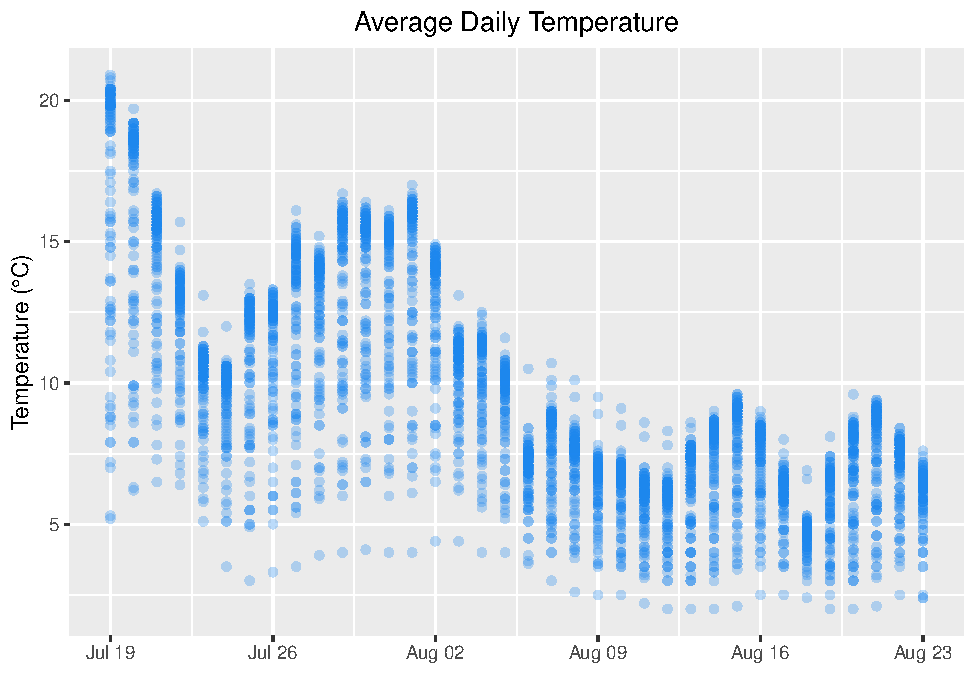
\includegraphics{iButtons1922Lanalysis_files/figure-latex/unnamed-chunk-16-1.pdf}

\begin{longtable}[]{@{}lr@{}}
\toprule\noalign{}
Veg Type & Mean Temp (°C) \\
\midrule\noalign{}
\endhead
\bottomrule\noalign{}
\endlastfoot
L2 & -4.1 \\
M1 & -5.4 \\
M3 & -4.5 \\
M3t & -4.1 \\
W1 & -3.8 \\
W2 & -4.3 \\
\end{longtable}

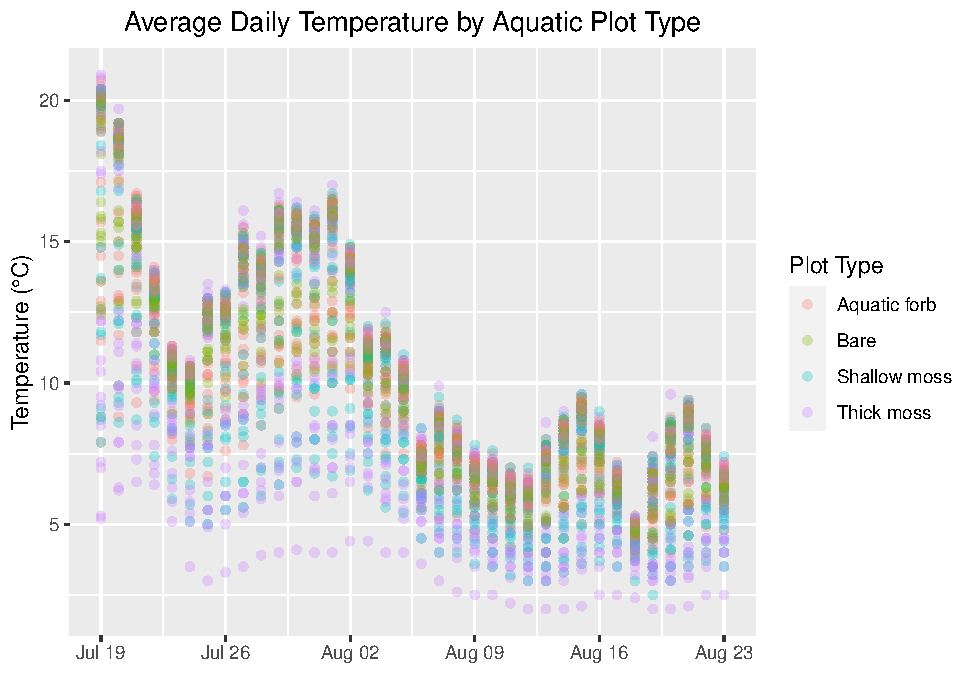
\includegraphics{iButtons1922Lanalysis_files/figure-latex/unnamed-chunk-19-1.pdf}

\begin{longtable}[]{@{}lr@{}}
\toprule\noalign{}
iBtn Position & Mean Temp (°C) \\
\midrule\noalign{}
\endhead
\bottomrule\noalign{}
\endlastfoot
L2 & -4.1 \\
M1 & -5.4 \\
M3 & -4.5 \\
M3t & -4.1 \\
W1 & -3.8 \\
W2 & -4.3 \\
\end{longtable}

\includegraphics{iButtons1922Lanalysis_files/figure-latex/unnamed-chunk-22-1.pdf}

\begin{longtable}[]{@{}lr@{}}
\toprule\noalign{}
Surficial Geology & Mean Temp (°C) \\
\midrule\noalign{}
\endhead
\bottomrule\noalign{}
\endlastfoot
Qsg & -4.6 \\
Qt & -4.3 \\
Qti & -4.2 \\
\end{longtable}

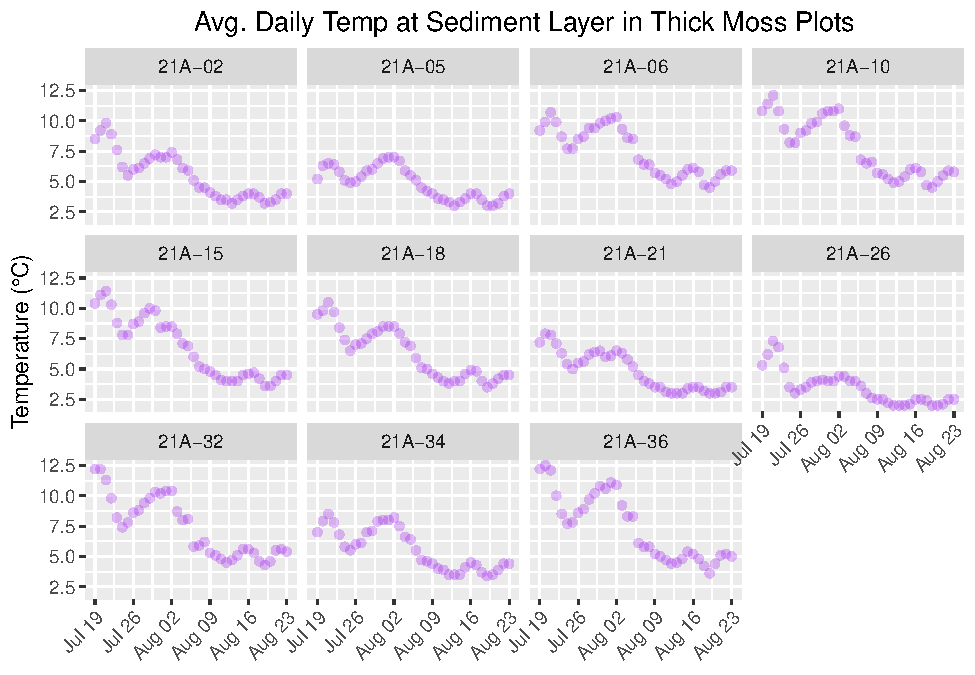
\includegraphics{iButtons1922Lanalysis_files/figure-latex/unnamed-chunk-23-1.pdf}

\begin{longtable}[]{@{}llr@{}}
\toprule\noalign{}
Veg Type & Surf Geol & Mean Temp (°C) \\
\midrule\noalign{}
\endhead
\bottomrule\noalign{}
\endlastfoot
L2 & Qti & -4.1 \\
M1 & Qsg & -5.5 \\
M1 & Qti & -4.6 \\
M3 & Qsg & -4.7 \\
M3 & Qti & -4.5 \\
M3t & Qsg & -4.1 \\
W1 & Qsg & -3.4 \\
W1 & Qti & -4.0 \\
W2 & Qt & -4.3 \\
W2 & Qti & -4.3 \\
!{[}{]}(iButton & s1922Lanalys &
is\_files/figure-latex/unnamed-chunk-24-1.pdf) \\
\end{longtable}

\begin{longtable}[]{@{}llr@{}}
\toprule\noalign{}
Veg Type & iBtn Position & Mean Temp (°C) \\
\midrule\noalign{}
\endhead
\bottomrule\noalign{}
\endlastfoot
L2 & Qti & -4.1 \\
M1 & Qsg & -5.5 \\
M1 & Qti & -4.6 \\
M3 & Qsg & -4.7 \\
M3 & Qti & -4.5 \\
M3t & Qsg & -4.1 \\
W1 & Qsg & -3.4 \\
W1 & Qti & -4.0 \\
W2 & Qt & -4.3 \\
W2 & Qti & -4.3 \\
\end{longtable}

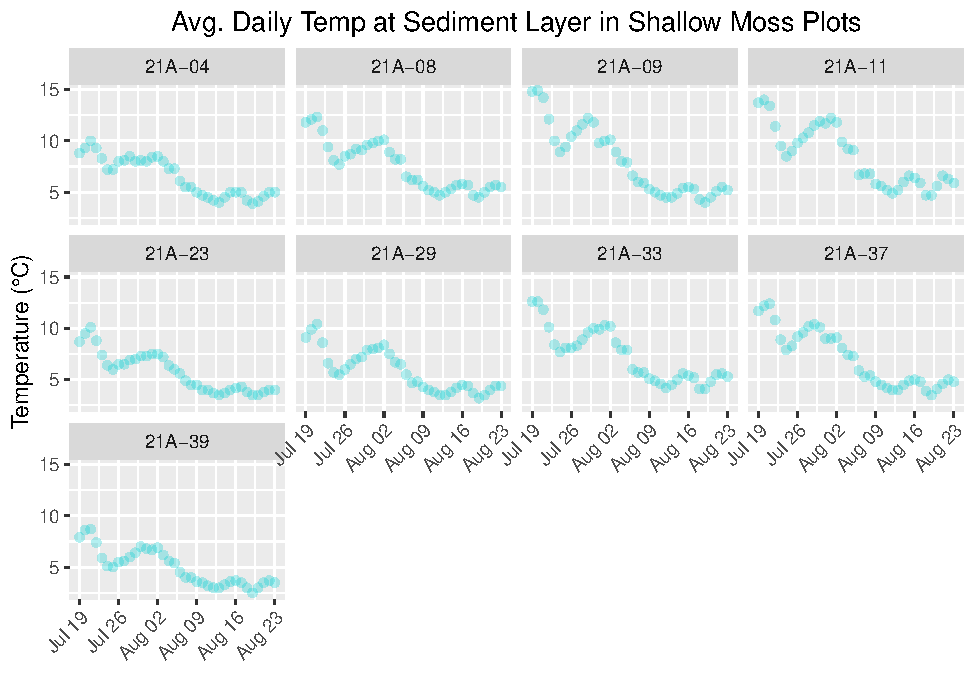
\includegraphics{iButtons1922Lanalysis_files/figure-latex/unnamed-chunk-25-1.pdf}

\subsubsection{Let's look at the data in more
detail.}\label{lets-look-at-the-data-in-more-detail.}

Here is a plot of the average daily temperature of each iButton from all
vegetation types at soil surface and the base of the organic layer.

\includegraphics{iButtons1922Lanalysis_files/figure-latex/unnamed-chunk-26-1.pdf}
Now we can look at the just the surface data colored to indicated the
vegetation type of the plot.

\includegraphics{iButtons1922Lanalysis_files/figure-latex/unnamed-chunk-28-1.pdf}
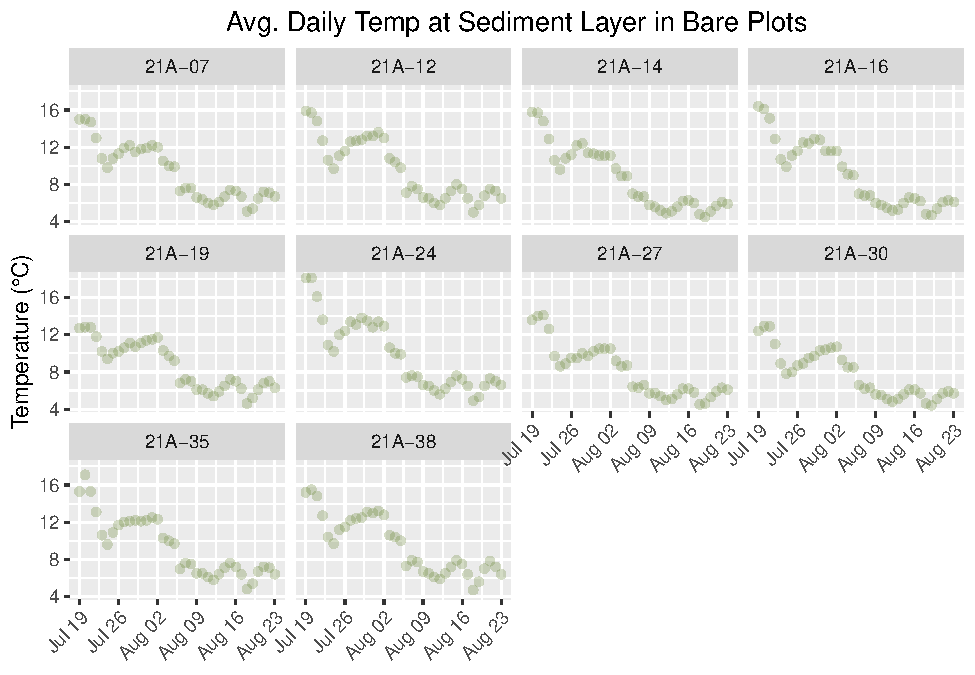
\includegraphics{iButtons1922Lanalysis_files/figure-latex/unnamed-chunk-29-1.pdf}
Now we can look at the just the base of the organic layer data colored
to indicated the vegetation type of the plot.

\includegraphics{iButtons1922Lanalysis_files/figure-latex/unnamed-chunk-31-1.pdf}

Here is a plot of the average daily temperature of each iButton by site
moisture

\includegraphics{iButtons1922Lanalysis_files/figure-latex/unnamed-chunk-32-1.pdf}

\includegraphics{iButtons1922Lanalysis_files/figure-latex/unnamed-chunk-33-1.pdf}

\includegraphics{iButtons1922Lanalysis_files/figure-latex/unnamed-chunk-34-1.pdf}

\includegraphics{iButtons1922Lanalysis_files/figure-latex/unnamed-chunk-36-1.pdf}

\subsubsection{That's it! (for now)}\label{thats-it-for-now}

\end{document}
